% Results
\section{Results}
Three curves were chosen to demonstrate the aspects of the developed 
methods. The first is a family of curves, $Lissajous$ curves 
(\Cref{fig:lissajous}), which are a combination of two perpendicular 
harmonic oscillations. This curve was chosen due to the sharp changes in 
curvature and self-intersecting nature, which are present in real-world 
applications. The second curve, a tricuspoid 
(\Cref{fig:tricuspoid}) was chosen for the sharp, discontinuous features, 
which are also present in real-world applications. 
In \Cref{fig:lissajous,fig:tricuspoid,fig:lastfigure} the curve is shown in red, and the discretization is shown in black with vertices highlighted by circles indicating their position. Each curve was scaled so that the parametrization, $t$, was normalized between zero and unity. In each case the curve was originally discretized using one segment corresponding to a vertex located at $t=0$ and $t=1$. Once the original discretization is created, the discretizations are refined using \Cref{alg:discreteoptimize}. Further results can be found in \Cref{tab:curvelength}. In this table, the true lengths of the curves can be found. The combined length of the segments in each discretization are also given with the actual arc-length deficit.
{\bf{Dave:  Add a sentence on the run time here.}}

\begin{figure}[h!]
  \centering
  \begin{tabular}{ccc}
  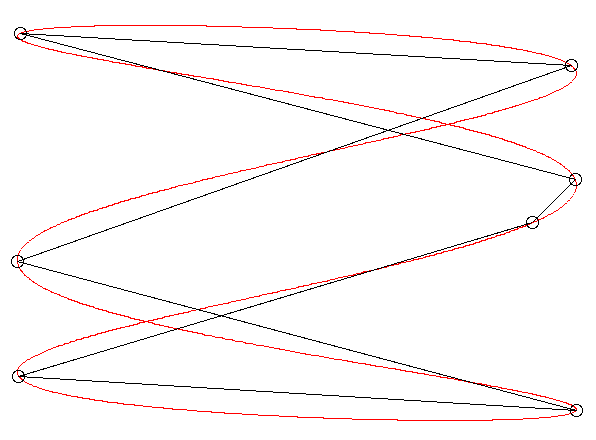
\includegraphics[width=0.3\linewidth]{Figures/lissajous01.png} &
  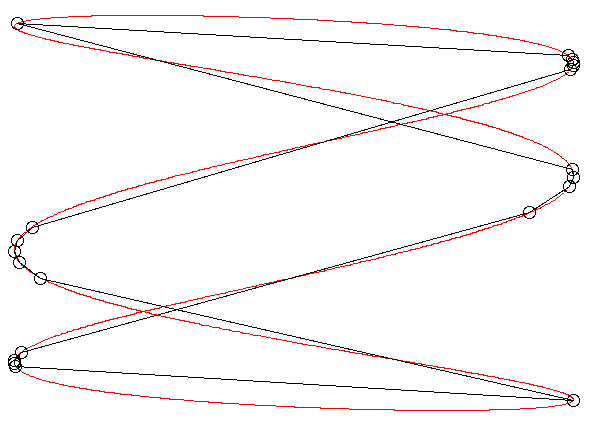
\includegraphics[width=0.3\linewidth]{Figures/lissajous001.png} &
  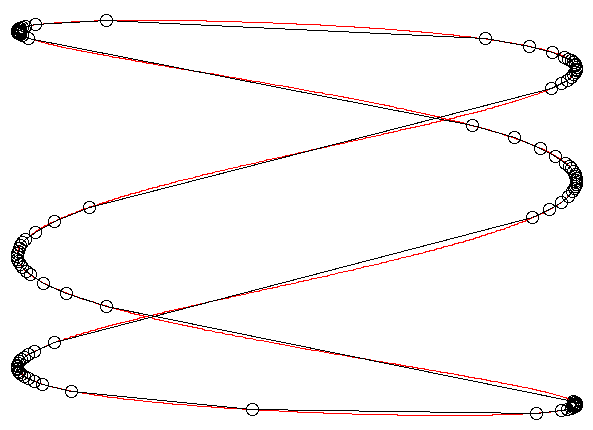
\includegraphics[width=0.3\linewidth]{Figures/lissajous0001.png}
  \end{tabular}
  \caption{\label{fig:lissajous} Lissajous Curves: 10\% deficit (left), 
1\% deficit (middle), 0.1\% deficit (right);\newline $x(t) = a * \sin(n*t 
+ c)$, $y(t) = b* \sin(t)$, $a=b=c=1$, $n=3$, $0 < t < 2\pi$}
\end{figure}

For the Lissajous curve, the optimization can be seen to be effective and 
efficient with regards to only generating vertices where the curvature is high and not wasting vertices on the relatively ``straight'' portions of the curve. In addition, the self-intersection present on this curve did not impede the generation of an optimal edge grid.

\begin{figure}[h!]
  \centering
  \begin{tabular}{ccc}
  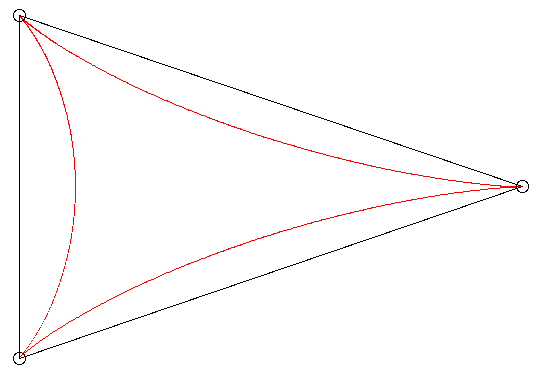
\includegraphics[width=0.3\linewidth]{Figures/tricuspoid01.png} &
  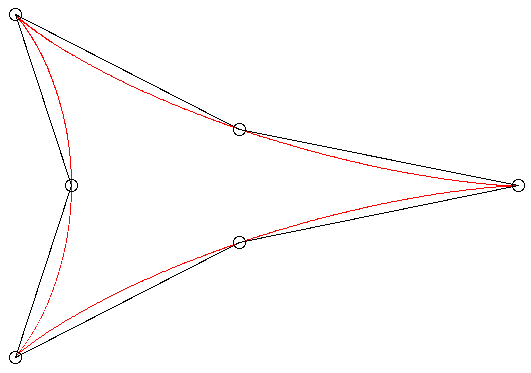
\includegraphics[width=0.3\linewidth]{Figures/tricuspoid001.png} &
  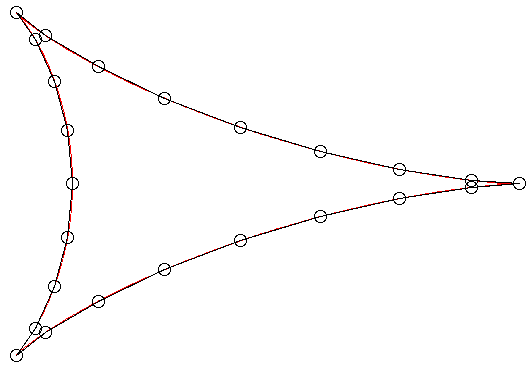
\includegraphics[width=0.3\linewidth]{Figures/tricuspoid0001.png}
  \end{tabular}
  \caption{\label{fig:tricuspoid} Tricuspoid Curve: 10\% deficit (left), 
1\% deficit (middle), 0.1\% deficit (right);\newline $x(t) = a*(2*\cos(t) 
+ \cos(2*t))$, $y(t) = a*(2*\sin(t) - \sin(2t))$, $a=1$, $0<t<2*\pi$}
\end{figure}

For the Tricuspoid curve, the optimization can be seen to be accurate with regards to placing a vertex at the discontinuities. Placing a vertex at the discontinuity is efficient since no further nodes are required to capture that feature of the curve. It can be seen that further refinements are placed elsewhere in order to capture curvature.

\begin{figure}[h!]
  \centering
  \begin{tabular}{ccc}
  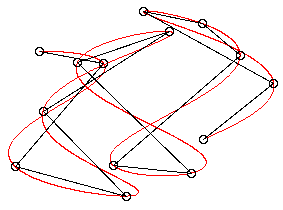
\includegraphics[width=0.3\linewidth]{Figures/random01.png} &
  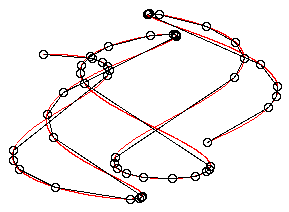
\includegraphics[width=0.3\linewidth]{Figures/random001.png} &
  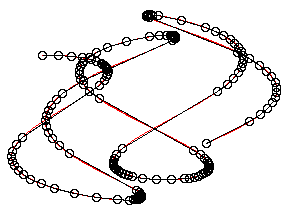
\includegraphics[width=0.3\linewidth]{Figures/random0001.png}
  \end{tabular}
  \caption{\label{fig:lastfigure} {\bf{Dave:  State which type of 
curve and fix line break if need be.}} Curve: 10\% deficit (left), 1\% 
deficit 
(middle), 0.1\% deficit (right);\newline $x(t) = 2*t + 3*\sin(7*t)$, $y(t) 
= t + 8*\cos(3*t)$, $0<t<1$}
\end{figure}

{\bf{Dave:  My first choice curve would be \#9, the cochleoid.  If it''s 
too tough to type the parametrization, then my second choice is \#16, the 
epicycloid.  The reason that I like \#9 is because the curves are becoming 
closer together near the self-intersection points.  The nice thing about 
\#16 is that it combines cusps with self-intersections.  The first two 
curves only have one or the other.}}
THIS CURVE IS REALLY SIMILAR TO THE LISSAJOUS CURVE BUT I PUT THE FIGURE AND THIS PARAGRAPH HERE TO SIMULATE A THIRD EXAMPLE IN ORDER TO GIVE AN ACCURATE PAGE COUNT. THIS CURVE IS REALLY SIMILAR TO THE LISSAJOUS CURVE BUT I PUT THE FIGURE AND THIS PARAGRAPH HERE TO SIMULATE A THIRD EXAMPLE IN ORDER TO GIVE AN ACCURATE PAGE COUNT. The numbers and results are real though if you like this curve better than the one above. I tried to find a ``more interesting'' curve but the equation would be too long to present here. I guess I could cite the formulation but it would be a lot of work programming up heavy-sided step functions, etc...

\Cref{tab:curvelength} summarizes the results from discretizing the three 
curves. Each row shows the results from a particular percentage change in edge length that was used as the refinement constraint. In each row is the discretization length of each curve is shown along with the arc-length deficit relative to the true length of the curve and number of segments in parenthesis. Each result is under the desired arc-length deficit for the entire curve -- except for 1\% result for the $Lissajous$ curve which is slightly higher. Other test results run by the authors showed similar results in accuracy and robustness.

\begin{table}[h!] \caption{\label{tab:curvelength} Discretization length 
with respect to true curve length.  {\bf{Dave:  What do 8, 21, and 121 
represent in first column of results?  Modify headers.}}} 
\begin{tabular}{cccc}
 & Lissajous Curve & Tricuspoid & last curve \\
True Length & 13.0653 & 16.0 & 108.938\\
10\% deficit & 12.7123 (2.7\%, 8) & 15.5885 (2.5\%, 4) & 102.875 (5.566\%, 14)\\
1\% deficit & 12.884 (1.4\%, 21) & 15.87 (0.78\%, 7) & 107.975 (0.8846\%, 51)\\
0.1\% deficit & 13.04 (0.166\%, 121) & 15.99 (0.058\%, 25) & 108.823 (0.105\%, 181)
\end{tabular}
\end{table}
